\documentclass[10pt,twocolumn]{article}

% Package

\usepackage{lipsum} % for generating filler tex
\usepackage{graphicx}
\usepackage[utf8]{inputenc}
\usepackage{geometry}
\usepackage{graphicx}
\usepackage{amsmath}
\usepackage{amsfonts}
\usepackage{amssymb}
\usepackage{multicol}
\usepackage{etoolbox} % For changing bibliography font size
\usepackage{titlesec}

% Set page geometr

\geometry{a4paper, margin=0.7in}

% Adjust spacing for section and subsection headings
\titlespacing*{\section}{0pt}{0.55\baselineskip}{0.55\baselineskip}
\titlespacing*{\subsection}{0pt}{0.5\baselineskip}{0.5\baselineskip}
\titlespacing*{\subsubsection}{0pt}{0.5\baselineskip}{0.5\baselineskip}

\begin{document}

% Title and author detail

\title{\textbf{Extraction and Visualization of Future-related Content From News Articles}}
\author{
    Juwal Regev\\
    Affiliation 1\\
    juwal.regev@student.uibk.ac.at
    \and
    Author Name 2\\
    Affiliation 2\\
    Email 2
}
\date{} % Remove date

\maketitle

\begin{abstract}
In today's rapidly evolving world, maintaining a comprehensive overview of the future landscape is essential for staying competitive and making informed decisions. However, given the overwhelming volume of daily news, manually obtaining a thorough overview of an entity's future prospects is quite challenging. To address this, we present a system that is designed to automatically extract future-related information of a queried entity from news articles. Our approach involves finetuning a language model on a novel multi-source dataset consisting of X annotated sentences to identify future-related sentences. We use topic modeling to extract the main topics from the data. These topics, along with their contents are subsequently ranked by relevance and presented on a timeline by identifying and resolving temporal expressions in the sentences using a temporal tagger. User evaluations have shown favorable feedback on the timelines and summaries our system produces.
\end{abstract}

\section{Introduction}
A vast amount of news articles is published on the web every single day. A significant amount of those articles contains information that is predictive or related to future events. Analyzing and extracting such information regarding a specific entity would offer a comprehensive overview of its future prospects.

\noindent However doing this manually is not feasible as one would have to sift through the articles line by line, identifying nuanced references to the future. Furthermore this would have to be done regularly as to always have the most up to date information. So it is clear that an automated system, capable of extracting, aggregating and visualizing this information is needed. This system would be beneficial in a variety of different fields. From analyzing predictions related to stock market movements, monitoring corporate developments as well as gaining insights into market trends and emerging technologies, the potential applications are limitless.

\noindent To address this problem, we present a system specifically designed for extracting, summarizing, ranking and visualizing future-related content within news collections. The process is initiated by a user providing an entity, whose future should be explored. The system then downloads and preprocesses thousands of news articles related to the provided entity. In the next step a neural network classifier is employed to classify sentences as either being future-related or not. Simply presenting the user a list of positive sentences doesn't offer a clear overview, especially when the text amount increases, and therefore they are clustered into distinct topics and presented to the user in a segmented manner. Additionally, the topics are labeled with representative keywords that provide insight into the content of each cluster. To provide an even better overview, we incorporate the temporal perspective into the presentation of the results. We do this by analyzing the sentences for temporal expressions, extracting and normalizing them to a date and then mapping the sentences onto a timeline. To convey the user the importance of a prediction, next to every sentence the number of times the sentence (and sentences similar to it) occurred in the corpus is shown.

\noindent In the following, we will delve into the system's architecture, providing implementation details, explaining the user interface and presenting the findings of a user study conducted to assess the system's result quality.

\section{Related Work}
Automatic identification and extraction of future-related information from text has been researched for decades. Baeza-Yates \cite{BaezaYatesSearchingTF} first formalized the concept of "future retrieval" . Early methods relied on time-taggers and predefined temporal expressions to extract data, but this resulted in limited diversity \cite{chronoseeker, supportingAnalysis, analyzingCollective, rankingRelated, extractingCollective}. Data was analyzed for unique properties \cite{improvingRetrieval} to create features for classifier training \cite{computationalExploration}.
For example, one study uses morphosemantic patterns as features \cite{automaticExtraction}, while another classifies clauses to determine if a sentence refers to the future, using features like POS tags and word co-occurrences \cite{extractingPredictive}. Some systems also predict future events using past data \cite{miningTheWeb, predictingTheNews}.
In Timeline Summarization, content is clustered and ranked to form a timeline. Techniques involve using TF-IDF-vectors or SBERT embeddings \cite{sbert} to represent sentences, and methods like Affinity Propagation \cite{abstractiveTimeline, multiTimeline} and Markov Clustering \cite{stateOfTheArtTimeline} for clustering. Sentence rankings inside of a topic or event often depend on the similarity to a centroid sentence \cite{stateOfTheArtTimeline} or on metrics like date-importance and informativeness \cite{abstractiveTimeline}.

In our work, we gather data manually, instead of using pre-defined queries or a temporal tagger, which enables us to accumulate a novel and more diverse dataset of future-related sentences. Our approach utilizes the power of language models for classificaton, clustering and ranking, to construct an intuitive end-to-end system.

\begin{figure*}[t]
\centering
% First image
\begin{minipage}{0.48\textwidth}
\centering
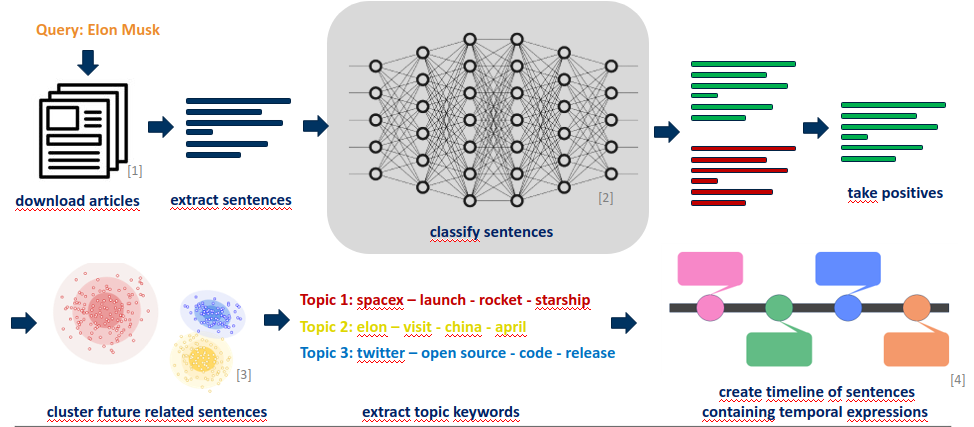
\includegraphics[width=9cm]{img/system.png}
\caption{Schematic Overview of the System Architecture.}
\label{fig:image1}
\end{minipage}
\hfill
% Second image
\begin{minipage}{0.48\textwidth}
\centering
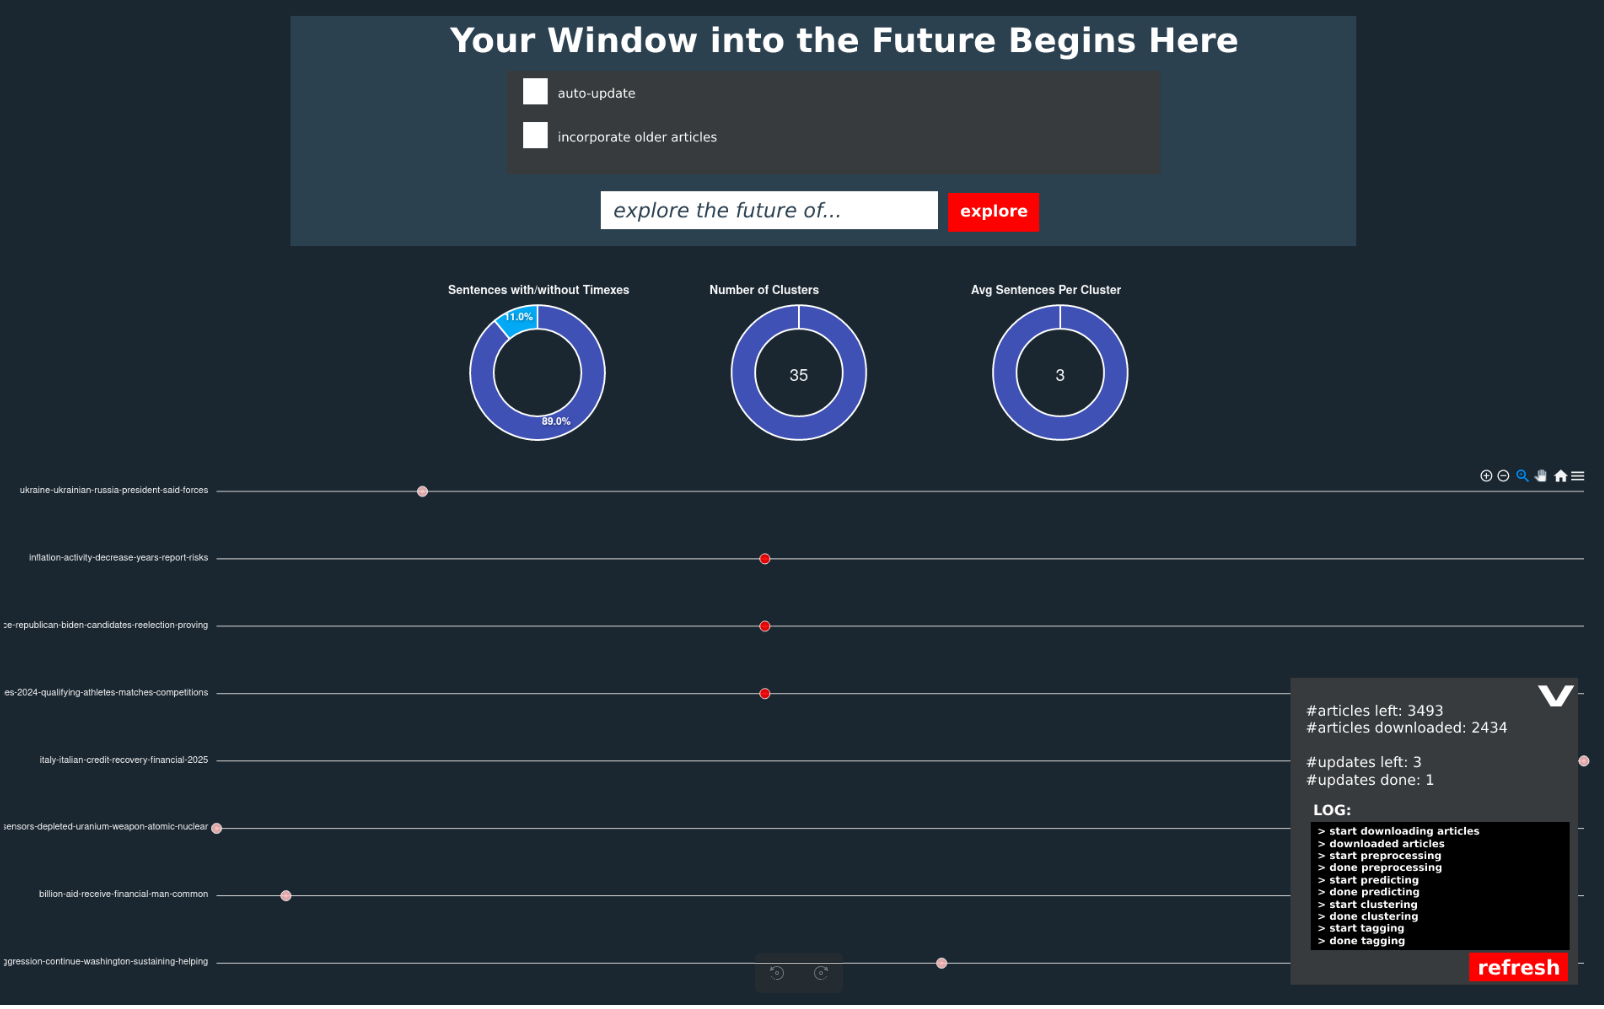
\includegraphics[width=9cm]{img/ui.png}
\caption{Timeline View with Settings and Statistics.}
\label{fig:image2}
\end{minipage}

\end{figure*}

\section{Dataset}
As already mentioned, our approach to data gathering differs from traditional methods. Earlier strategies have frequently relied on extracting data using temporal expressions, however this approach has its limitations. Predictions can often be intricate, lacking explicit dates or simple temporal cues.
To address this, our dataset incorporates a rich variety of X manually labeled sentences. They have been collected from different sources, and therefore they contain a diverse set of topics, and exhibit unique lexical and structural features. This makes our classifier be able to identify future-related content that does not contain standard temporal expressions hinting at future references.
Here's a breakdown of our data sources: predictions from platforms such as Longbets and Horizons, where users can upload predictions, sentences generated via ChatGPT \footnote{https://openai.com/gpt-4} and sentences from news collections. The majority of sentences stem from news articles.


\subsection{System Overview}
Our system consists of five main components: 1) Fetching and Preprocessing, 2) Classification, 3) Topic Modeling, 4) Postprocessing, 5) Time-Tagging.

In the following sections, we will explore each component in depth, gaining a detailed understanding of the overall workflow and examining implementation details.

\subsubsection{Fetching and Preprocessing}
To initiate the process, the user has to provide a query to the system, which can take the form of a topic, an entity, or any other input whose future should be analyzed. The user has the option to determine the number of articles that should be downloaded, as well as the time frame from which these articles should be fetched. Once the articles are downloaded, they are split up into their constituent sentences. These sentences subsequently undergo preprocessing in order to prepare them for the next steps.

\subsubsection{Classification}
Our classifier was implemented using a DistilRoBERTa model \footnote{https://huggingface.co/distilroberta-base}, which was fine-tuned by appending a standard feed-forward network to the output. DistilRoBERTa is a smaller, faster version of the renowned RoBERTa language model \cite{roberta}, trained to preserve its performance on downstream tasks. It was chosen over the larger RoBERTa model because our system requires real-time inference, where speed is critical. To further increase performance, the sequence length was reduced to 50 tokens, a significant reduction from the default 512 sequence length. Since the model only takes one sentence at a time, and the average English sentence consists of about 15-20 words, this should still be more than enough.
DistilRoBERTa produces an embedding for each token, but since we want to classify the entire sentence, we need a single embedding vector to represent it. We could simply append the vectors to form a large sentence embedding vector, but a more efficient method is mean-pooling, which takes the average of the word embeddings to obtain a smaller vector that captures the general semantic information of the entire sentence. This also reduces the size of the finetuning feed-forward network, which then only takes a 512-dimensional vector as input.

\paragraph{Training Insights}
We finetuned the network on the X sentence-dataset for X epochs with the following configurations:
	- Batch size: X
	- Learning rate: X
	- Warmup: X
	- Weight decay: X
These optimal configurations were identified through 5-fold cross-validation on the dataset.

\paragraph{Validation}
\textbf{TODO}

\paragraph{Inference}
The preprocessed sentences are fed into the fully trained model, which outputs a score between 0 and 1, indicating the probability that the sentence is future-related. All sentences with a probability above 0.9 are returned as positives. To enable active learning, all sentences are stored with their confidence scores, manually labeled and inserted into the training dataset.

\subsubsection{Topic Modeling}
To present the user with sentences assigned to topics, we perform topic modeling using BERTopic, a system that extracts topics from text documents by embedding them in a high-dimensional space using SBERT and then clustering the embeddings by similarity.
It also extracts representative keywords from the topics, which are used as topic-headings. We configured BERTopic to perform dimensionality reduction with UMAP and clustering with HDBSCAN.

\subsubsection{Postprocessing}

To enhance the results of topic modeling, we postprocess the results in two ways.
First, we ensure that the sentences are relevant enough to their assigned topic, by matching the topic keywords against the words in each sentence. If a sentence contains fewer than three topic keywords, it is removed from the dataset.
The next step aims for eliminating redundancy within a topic. Using the previously generated SBERT sentence embeddings from the topic modeling step, we calculate the cosine similarity between all sentence pairs within the same topic. When two sentences have a cosine similarity above 0.8, they are considered duplicates. Each sentence is assigned a count of its exact and approximate duplicates within its assigned topic. Finally, the sentences' cosine similarity scores are compared and if two similar sentences are identified, the one with the higher duplicate count is retained and the other is discarded.

This step ensures that clusters remain diverse, avoiding redundancy that might arise from differently formulated sentences discussing the same information.

\subsubsection{Time-Tagging}
To create a timeline, we need to map sentences to concrete dates. This requires the identification and resolution of temporal expressions in the sentences. The SUTime time-tagger \cite{sutime} was employed for this purpose. It detects temporal information and resolves it to the referenced date, incorporating the article's publication date.
Some rules had to be added to ensure that all temporal expressions are mapped to dates, such as mapping 'Summer' to '15.08'.
While the tagger generally performs well, there are some problems with ambiguous references like 'On Tuesday, he revealed his decision, which will become official soon.'
The time-tagger maps "on Tuesday" to the coming Tuesday, which is in the future, even though the sentence is referring to a past event. This is a known limitation of SUTime and is mitigated by simply discarding extracted temporal expressions that reference weekdays.

\subsection{Demonstration System}
The system was implemented as a webapp that can be accessed with a standard browser. Due to the workflow taking a significant amount of time, the whole process is executed multiple times, each time downloading new articles, classifying them and then clustering them together with the previously extracted sentences. When new results are ready, a button appears, which lets the user give permission to load in the updated data.

\subsubsection{Settings}
Upon entry, the website shows a settings panel which provides the user with some adjustable configurations. Here, decisions about whether updates should be automatic or manual can be made. There's also the possibility to specify the quantity of articles and their time frame. A text field prompts users to specify an entity for exploration, with a button to initiate the process.

\subsubsection{Statistics}
A statistics section is available, putting the data in numbers. Here, users can see the fraction of sentences which contain temporal expressions, get insights into the number of topic clusters, and see the average number of sentences per cluster.

\subsubsection{Timeline}
The website's core component is the timeline visualization. On this timeline, the y-axis shows the different topics, whereas the x-axis displays future dates referenced by the sentences. A data point on the timeline represents a collection of sentences belonging to the same topic, that all reference the same date. This collection of sentences is revealed when hovering over the datapoint in the form of a tooltip section. They are ranked according to their relevance score, which is also displayed next to each sentence. There is also an opportunity to delve into the full article for more context, by simply clicking on a sentence. The data point itself has a color assigned to it, representing the relevance of the sentences it contains, with brighter colors indicating higher relevance.

\subsubsection{Word Cloud}
Complementing the timeline is the Word Cloud, that provides the user with sentences that don't contain any temporal expressions. Each topic is represented as a cloud, whose size corresponds to the mean relevance of the contained sentences. On interaction, these clouds unfold to reveal the associated sentences again along with relevance score, and links to their origin articles.

%\subsubsection{Log View}
%There is also a log-view that can be expanded which gives the user an offer on the retrieval status. It enumerates articles fetched, details updates processed and pending, and lists out backend logs.

\section{Evaluation}
To assess the effectiveness of our system, we developed a six-task exercise and presented it to six different users. Each user had to complete the exercise with one of three entities, which were distributed evenly among the users. This means that two users always had the same exercise with the same entity.
These tasks were designed to examine the two core features of our system: the timeline and the word cloud. 
The tasks included: summarizing what's in store for an entity in the next 5 years, determining which topic and date have the highest/lowest relevance and to analyze the overall ranking, engaging with the timeline to find incorrectly resolved temporal expressions, summarizing the content of the most relevant word cloud, examine the word clouds for duplicate content and examining both components for sentences without future-related content.

The users provided lengthy summaries, implying a wide range of predictions for upcoming years. The color-coding of datapoints managed to successfully convey relevance, but users noticed that nearer predictions were generally marked as more relevant, while key distant predictions often had lower relevance scores. Some users found this to be a problem, as distant events are often more serious and require more time to unfold. The time-tagging was generally accurate, but struggled with some past predictions like "In 2019, he correctly predicted that a pandemic would occur by the end of the year.". This is because the tagger resolves temporal expressions relative to the parent-article's publishing date, and does not understand that "in 2019" should be the anchor date. Some users found similar sentences in the same cluster, but the information they provided was slightly different. This provided additional context, which was well-received.

Overall, users were satisfied with the system, particularly with its ability to provide a clear and comprehensive overview of an entity's future plans, events, and decisions. However, the biggest critique was the system's speed, especially the time it takes to retrieve the initial results. This should be reduced.


\section{Conclusions}
By developing a multi-source dataset of X labeled sentences, we trained a DistilRoBERTa model to identify future references.  We then used BERTopic for topic modeling and SUTime for time-tagging to extract topics from the data, detect and resolve temporal expressions. A dedicated post-processing step improved cluster quality and ranked sentences according to their relevance. We also designed an intuitive interface that presents the results with an interactive timeline and word clouds. A user study confirmed the system's ability to offer a detailed overview of the future, while also highlighting potential areas for improvement, especially speed.




% Generate the bibliography section
\small
\bibliography{lit}
\bibliographystyle{unsrt}

\end{document}

